\documentclass{llncs}
\usepackage{times}
\usepackage[portuguese]{babel}
\usepackage[utf8]{inputenc}
\usepackage[T1]{fontenc}

\usepackage{a4}
%\usepackage[margin=3cm,nohead]{geometry}
\usepackage{epstopdf}
\usepackage{graphicx}
\usepackage{fancyvrb}
\usepackage{amsmath}
%\renewcommand{\baselinestretch}{1.5}

\graphicspath{{./imagens/}}

\usepackage{url}
%\usepackage[colorlinks=true,linkcolor=blue,citecolor=blue]{hyperref}

\setlength\parindent{0pt}

\usepackage{listings}
%LISTING - GENERAL
\lstset{
  language=java,
	basicstyle=\scriptsize,
	numbers=left,
	tab=,
	tabsize=2,
	numberstyle=\tiny,
	numbersep=5pt,
	breaklines=true,
  frame=tB
}


\begin{document}
\mainmatter
\title{Comunicações por Computador --- Trabalho Prático 2}
\subtitle{Desenho e Implementação de um Jogo Distribuído na Internet}
\titlerunning{CC-TP2}
\author{Rui Camposinhos \and Carlos Rafael Antunes \and Nuno Oliveira}
\authorrunning{Camposinhos R. \and Antunes C. \and Oliveira N.}
\institute{
Universidade do Minho, Departamento de  Informática, 4710-057 Braga, Portugal\\
e-mail: \{a72625, a67711, a67649\}@alunos.uminho.pt
}
\date{}
\maketitle

\begin{abstract}
O presente relatório descreve a implementação de um jogo multi-utilizador online, com 
questões sobre músicas reproduzidas em tempo real. Foi implementada uma arquitectura 
com um servidor e multi-utilizadores, conectados numa rede local e com troca de datagramas UDP.
\end{abstract}

\section{Introdução}
No presente trabalho pretende-se implementar um jogo multi-utilizador online, com 
questões sobre músicas reproduzidas em tempo real.\\

Pretende-se implementar um sistema distribuído, com comunicações TCP entre servidores e 
comunicações UDP entre clientes e servidores, que procure optimizar a utilização da 
largura de banda, por transmissão selectiva, fiável e com controlo de fluxo e de erros 
(figura \ref{fig:arq}).

\begin{figure}
\begin{center}
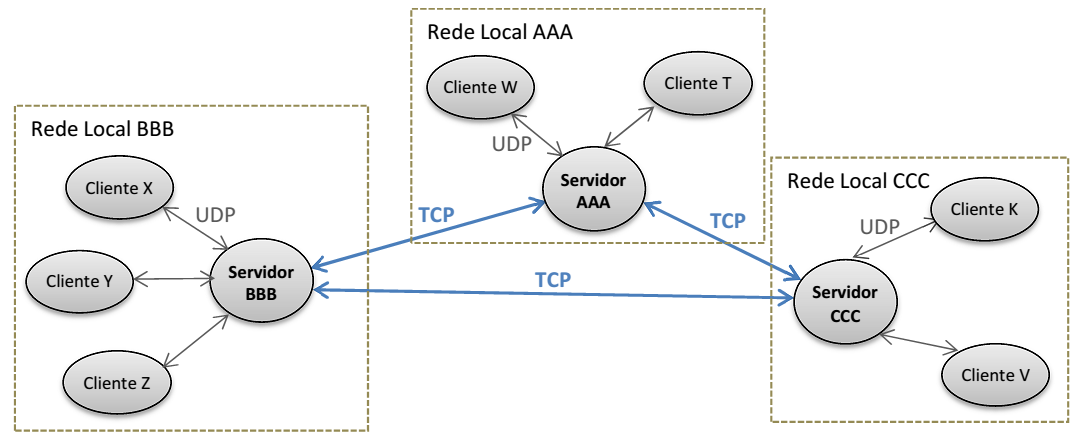
\includegraphics[width=10cm]{arq.png} 
\end{center}
\caption{Arquitetura do sistema a implementar (de acordo com o enunciado \cite{enun})}
\label{fig:arq}
\end{figure} 

\section{Hipóteses Alternativas ao Enunciado}
De uma forma geral foram adoptadas todas as hipóteses referidas no enunciado, 
salvo raras excepções.\\

Seguidamente listam-se algumas das alterações implementadas:
\begin{itemize}
\item No ficheiro de base de dados foi adoptado um separador diferente para os campos. 
		Alternativamente à vírgula (",") foi adoptado um ponto e vírgula (";"), de forma a 
		evitar conflitos com o texto que pudesse incluir vírgulas.
\item Nos tipos de pedidos dos clientes para os servidores, foi ignorado o pedido 
		\verb!RETRANSMIT!, tendo-se em alternativa implementado um pedido \verb!TRANSMIT!, 
		com o número da resposta pretendido.
\item No pedido \verb!ACCEPT_CHALLENGE! é devolvida a data e hora do desafio, em alternativa 
		a um simples \verb!OK!.
\item Foram acrescentados dois campos aos tipos de resposta dos servidores para os clientes: 
		Campo 19 - definido como uma etiqueta (tag) do PDU para dados gerais;
		Campo 30 - definido com \verb!NEXT_PACKAGE! (pacote esperado).
\end{itemize}

\section{Implementação}
Todo o código desenvolvido para o presente projecto foi realizado com a linguagem de 
programação \emph{java}.\\

Foram utilizadas várias bibliotecas auxiliares, sendo de destacar a biblioteca 
\verb!java.net! e em particular a classe \verb!DatagramPacket! 
\footnote{\url{http://download.java.net/jdk7/archive/b123/docs/api/java/net/DatagramPacket.html}}, 
utilizada para criar conexões do tipo UDP.

\subsection{Arquitectura do Sistema}
Para o presente projecto foram desenvolvidas duas aplicações:
\begin{enumerate}
\item Uma aplicação para clientes, designada \verb!TP2-CC-MusicClient!.
\item Uma aplicação para servidores, designada \verb!TP2-CC-MusicServer!.
\end{enumerate}

Não foi possível concluir a etapa de implementação das ligações TCP multi-servidor. 
Assim, a arquitectura do sistema implementada permite unicamente uma única instância de 
servidor (uma única rede local), com vários clientes a este conectados. As ligações 
cliente/servidor são todas realizadas por UDP.

\subsection{Estruturas de Dados}
As principais estruturas de dados implementadas foram: \verb!Campo!, \verb!ListaCampos! e
\verb!PDU!.

Para tal foram criadas classes, com o mesmo nome, que seguidamente se detalham.

\begin{lstlisting}[caption={Classe Campo}, label={code:campo}]
public class Campo {
    private byte tag; /*numero do tipo de resposta*/ 
    private int size; /* tamanho dos dados*/
    private byte[] dados; /* array de dados*/
}
\end{lstlisting}

\begin{lstlisting}[caption={Classe ListaCampos}, label={code:ListaCampos}]
public class ListaCampos {
    private ArrayList<Campo> lista; /*lista com todos os campos da mensagem a enviar*/
}
\end{lstlisting}

\begin{lstlisting}[caption={Classe PDU}, label={code:PDU}]
public class PDU {
    private byte versao; /*codigo da versao - por omissao 0*/
    private byte seguranca; /*seguranca - por omissao 0*/
    private short label; /*identificacao do pedido*/
    private byte tipo; /*codigo do tipo de pedido - ex:0->REPLY*/
    private byte nCampos; /* numero de campos seguintes*/
    private int tamanho; /*tamanho da lista de campos*/
    private byte[] lista; /*lista de campos*/
}
\end{lstlisting}


\subsection{Outros Detalhes}
De forma a controlar o fluxo entre servidor e clientes foi implementada uma 
estratégia de comunicação do tipo Stop-and-Wait, i.e., após envio de um pacote, 
o servidor espera confirmação do cliente para envio do pacote seguinte. Trata-se 
de uma técnica simples, mas que permite um controlo eficaz. De forma a ultrapassar 
as situações de erro (pacotes/confirmações perdidas) foi implementado um controlo 
por Time-Out no cliente. Após enviar uma confirmação, o cliente espera 20s pelo 
próximo pacote. Caso não o receba, reenvia confirmação de forma a forçar o reenvio 
do pacote perdido.\\

A escolha dos desafios pelo servidor é efectuada de forma aleatória. 
Sempre que é criado um desafio novo pelo cliente, o servidor escolhe de forma aleatória 
um dos desafios contidos na sua base de dados.\\

.........em curso..........
Divide-se o pdu gigante em fracções, e encapsulam-se usando outros PDUs.\\

Tamanhos passam a ser em int, em vez de short... short não aguenta o tamanho da musica...\\
.........em curso..........

\section{Testes e Resultados}
A aplicação dos clientes é corrida em ambiente shell, com recurso a menus de opções. 
Seguidamente apresentam-se alguns outputs do cliente e servidor.

\begin{multicols}{2}{
\scriptsize
Inicializaçao do Cliente:
\begin{verbatim}
*** CC-Music ***

*** Menu Principal ***

1-Login
2-Registar
0-Sair

Opçao: 
\end{verbatim}

Registo de novo utilizador:
\begin{verbatim}
*** Registar ***

Introduza os seus dados:
Nickname: rui
Password: pass
Nome: rui pedro
Enviado!
Resposta recebida!
OK!
\end{verbatim}

Resposta do servidor:
\begin{verbatim}
**Pacote de dados n.1 **

Versao correta.
Sem segurança.
Label: 1
Tipo: REGISTER
    Novo utilizador:
      Alcunha: rui
      Pass: pass
      Nome: rui pedro
Resposta enviada!

**Pacote de dados n.1 tratado **
\end{verbatim}

Login do cliente:
\begin{verbatim}

*** Login ***


Nickname: rui
Password: pass
Enviado!
Resposta recebida!
Bem vindo rui pedro!
\end{verbatim}

Resposta do servidor:
\begin{verbatim}
**Pacote de dados n.2 recebido **

Versao correta.
Sem segurança.
Label: 2
Tipo: LOGIN
    Login:
      Alcunha: rui
      Pass: pass
IP Recebido: /127.0.0.1 Port: 54029
Resposta enviada!

**Pacote de dados n.2 tratado **
\end{verbatim}

Menu Principal Cliente:
\begin{verbatim}
*** CC-Music ***

*** Menu Principal ***

1-Criar novo desafio
2-Listar os desafios atuais
3-Entrar num desafio
0-Sair

Opçao: 
\end{verbatim}

Novo desafio:
\begin{verbatim}
*** Criar novo desafio ***

Introduza o nome do desafio: teste
Introduza a data (AAMMDD): 150608
Introduza a hora (HHMMSS): 180000
Enviado!
Resposta recebida!
Desafio criado!
À espera que o desafio começe...
Tempo de Espera: 443 segundos...
Tempo de Espera: 442 segundos...
\end{verbatim}

Resposta do servidor:
\begin{verbatim}
**Pacote de dados n.4 recebido**

Versao correta.
Sem seguranca.
Label: 4
Tipo: MAKE_CHALLENGE
Desafio escolhido: 1
A ler o ficheiro desafio-000001.txt
Ficheiro lido com sucesso!
Novo desafio criado: teste
Resposta enviada!
**Pacote de dados n.4 tratado **
\end{verbatim}

Envio da pergunta 1 do desafio pelo servidor:
\begin{verbatim}
**Pacote de dados n.5 recebido **

Versao correta.
Sem segurança.
Label: 5
Tipo: TRANSMIT
Pedido para a pergunta 1 do desafio "teste".
Pergunta: Quem canta esta cancao?
Respostas: 
[Robert Smith, Bono Vox, Ninguem, 
     e uma musica instrumental] 
Resposta Certa: 3
Path da Imagem: 000001.jpg
Path da Musica: 000001.mp3
Tamanho da imagem: 105039
Imagem transformada em array de bytes!
Tamanho da imusica: 2411752
Musica transformada em array de bytes!
PDU criado!
A dividir em PDU's mais pequenos...
Número de pacotes: 52 Tamanho do PDU: 2516927
A guardar os pacotes na matriz...
Concluido!
Pacotes divididos com sucesso!
Resposta enviada!

**Pacote de dados n.5 tratado **
\end{verbatim}
}
\end{multicols}


\section{Conclusão e Trabalho Futuro}
No presente trabalho foram discutidas as principais questões relacionadas com a 
implementação de uma comunicação servidor-cliente, por intermédio de UDP. 
Foram descritas as estratégias adoptadas, o controlo de erros e de fluxo, 
os tipos de estruturas de dados utilizadas e apresentados alguns exemplos de aplicação.\\

%Trabalho futuro
Devido a dificuldades relacionadas com o prazo de entrega do trabalho, não foi possível 
completar alguns dos objectivos propostos, designadamente:
\begin{itemize}
\item Não foi possível implementar conexões multi-servidores através de TCP.
\item Não foi possível ultrapassar algumas dificuldades relacionadas com a 
	partição dos PDUs de maior tamanho, por exemplo no envio de músicas.
\item Não foram implementadas todos os tipos de resposta do servidor.
\end{itemize}

De referir também, que o protocolo de controlo de fluxo poderia ser melhorado através da 
utilização de uma janela deslizante, optimizando o número de mensagens trocadas entre 
servidor e cliente.

\section*{Acknowledgments}
O presente trabalho foi realizado no âmbito da unidade curricular de Comunicações por Computador, 
ano lectivo de 2014/2015, da Licenciatura em Engenharia Informática, da Universidade do Minho.

\bibliographystyle{splncs}
\bibliography{CC-2015-TP2-CamposinhosAntunesOliveira}

\end{document}
